% Options for packages loaded elsewhere
\PassOptionsToPackage{unicode}{hyperref}
\PassOptionsToPackage{hyphens}{url}
%
\documentclass[
]{book}
\usepackage{lmodern}
\usepackage{amssymb,amsmath}
\usepackage{ifxetex,ifluatex}
\ifnum 0\ifxetex 1\fi\ifluatex 1\fi=0 % if pdftex
  \usepackage[T1]{fontenc}
  \usepackage[utf8]{inputenc}
  \usepackage{textcomp} % provide euro and other symbols
\else % if luatex or xetex
  \usepackage{unicode-math}
  \defaultfontfeatures{Scale=MatchLowercase}
  \defaultfontfeatures[\rmfamily]{Ligatures=TeX,Scale=1}
\fi
% Use upquote if available, for straight quotes in verbatim environments
\IfFileExists{upquote.sty}{\usepackage{upquote}}{}
\IfFileExists{microtype.sty}{% use microtype if available
  \usepackage[]{microtype}
  \UseMicrotypeSet[protrusion]{basicmath} % disable protrusion for tt fonts
}{}
\makeatletter
\@ifundefined{KOMAClassName}{% if non-KOMA class
  \IfFileExists{parskip.sty}{%
    \usepackage{parskip}
  }{% else
    \setlength{\parindent}{0pt}
    \setlength{\parskip}{6pt plus 2pt minus 1pt}}
}{% if KOMA class
  \KOMAoptions{parskip=half}}
\makeatother
\usepackage{xcolor}
\IfFileExists{xurl.sty}{\usepackage{xurl}}{} % add URL line breaks if available
\IfFileExists{bookmark.sty}{\usepackage{bookmark}}{\usepackage{hyperref}}
\hypersetup{
  pdftitle={CalcZ Student Notes},
  pdfauthor={Daniel Kaplan},
  hidelinks,
  pdfcreator={LaTeX via pandoc}}
\urlstyle{same} % disable monospaced font for URLs
\usepackage{longtable,booktabs}
% Correct order of tables after \paragraph or \subparagraph
\usepackage{etoolbox}
\makeatletter
\patchcmd\longtable{\par}{\if@noskipsec\mbox{}\fi\par}{}{}
\makeatother
% Allow footnotes in longtable head/foot
\IfFileExists{footnotehyper.sty}{\usepackage{footnotehyper}}{\usepackage{footnote}}
\makesavenoteenv{longtable}
\usepackage{graphicx}
\makeatletter
\def\maxwidth{\ifdim\Gin@nat@width>\linewidth\linewidth\else\Gin@nat@width\fi}
\def\maxheight{\ifdim\Gin@nat@height>\textheight\textheight\else\Gin@nat@height\fi}
\makeatother
% Scale images if necessary, so that they will not overflow the page
% margins by default, and it is still possible to overwrite the defaults
% using explicit options in \includegraphics[width, height, ...]{}
\setkeys{Gin}{width=\maxwidth,height=\maxheight,keepaspectratio}
% Set default figure placement to htbp
\makeatletter
\def\fps@figure{htbp}
\makeatother
\setlength{\emergencystretch}{3em} % prevent overfull lines
\providecommand{\tightlist}{%
  \setlength{\itemsep}{0pt}\setlength{\parskip}{0pt}}
\setcounter{secnumdepth}{5}
\ifluatex
  \usepackage{selnolig}  % disable illegal ligatures
\fi

\title{CalcZ Student Notes}
\author{Daniel Kaplan}
\date{2021-05-14}

\begin{document}
\maketitle

{
\setcounter{tocdepth}{1}
\tableofcontents
}
\hypertarget{status}{%
\chapter*{Status}\label{status}}
\addcontentsline{toc}{chapter}{Status}

This is the working version for Summer 2021.

\hypertarget{part-block-2-differences-and-differentiation}{%
\part{Block 2: Differences and differentiation}\label{part-block-2-differences-and-differentiation}}

\hypertarget{functions-and-patterns}{%
\chapter{Functions and patterns}\label{functions-and-patterns}}

As you know, a function takes one or more inputs and returns a value as output. The functions we examine in CalcZ take \emph{quantities} as inputs and return a \emph{quantity} as an output.
The algorithm that forms the body of the function describes arithmetic and other calculations that can turn the inputs into the output.

On the other hand, we can also use \textbf{\emph{tables}} as functions. With a table, you specify the input, look up that input in one of the colums of the table which brings you to the right row. Then read out from that row the value in another column to be the output. The quantitative operation needed for table lookup is simple comparison. The floor/corridor/door metaphor describes table lookup as well as function evaluation.

In the previous block, we constructed functions to represent the patterns seen in data. In one example, we constructed a function \(g(t) = A + B e^{-k t}\) to represent the temperature of water cooling in a mug as a function of time. In another example, we summarized the pattern of rising and falling tides.

It's common sense that data is stored in tables. But we could easily represent any smooth mathematical function, such as our basic modeling functions, as a table look-up problem. Indeed, in the era before computers, many mathematical functions were used in exactly this manner: a printed table in which a person could search for a match to the input and retrieve a value for the output.

{[}Picture of some nice old table.{]}

In the computer era, we still routinely represent functions this way: data stored in computer files. For instance, an MP3 file is not much more than a sequence of numbers that record a complicated function of time: the air pressure variations of sound. Similarly, digital images record functions of \(x\) and \(y\) over a limited domain. Given \(x\) and \(y\) as input, you can look up the output by going to the right pixel.

We humans of course, don't perceive the numerical output of either sound or image functions: we \textbf{hear} a sound and we \textbf{see} an image. We've got special biological equipment for this!

Consider the image in Figure @ref\{fig:sand-1\}. It is a picture of some indentations in a small area of sand, about two inches wide in the middle of a hiking trail. The dots are individual grains of sand.

\begin{center}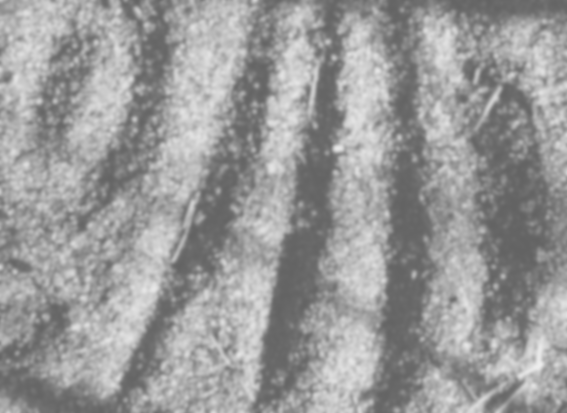
\includegraphics[width=0.5\linewidth]{www/sand-furrows} \end{center}

Can you see three almost parallel furrows? How about the small crater in the upper left?

You can see the individual grains of sand because they contrast sharply with their neighbors. Or, more precisely, you can see a few dozen grains \textbf{because} they contrast sharply with their neighbors.

You can think of the surface of the sand as a function of \(x\) and \(y\). It's lower in some places and higher in others. But, in fact, you can't see the height of an individual point in the photograph. In the right light, you wouldn't notice the furrows at all. But the way the picture is lighted, raking sunlight from the left, the surface is translated into broad regions of brightness and shadow. In the light regions, the surface slants toward the sun. In the shadows, the surface slants away from the sun.

What you're mainly seeing in the photo is the \textbf{\emph{slant}} or \textbf{\emph{slope}} of the surface. The light has transformed \emph{elevation} as a function of \(x\) and \(y\) into \emph{slant} as a function of \(x\) and \(y\) and then encoded the slant as brightness, in much the same way the background of a contour plot encodes the output of the function as a color.

The moral here is that sometimes the data in a function is not in the right form for us to extract useful information. But by transforming that data to represent contrast or difference or slope, the information can be revealed.

This Block is about transforming functions to show difference and slope. Such transformation, accomplished by mathematics rather than the raking light of the sun, can take a pattern that we're presented with and turn it into another pattern that can tell us what we want to know.

\hypertarget{average-rate-of-change}{%
\section{Average rate of change}\label{average-rate-of-change}}

\begin{enumerate}
\tightlist
\item
  \textbf{{[}Deriv-2a{]}} \emph{Identify the ``average rate of change'' of a function over an interval as the overall change in output divided by the change in input.}
\end{enumerate}

As you know, one way to calculate the slope of a straight-line function \(f()\) is to pick two different values for the input: call the larger of them \(x_1\) and the smaller \(x_0\). Think of these input values as the endpoints of an \textbf{\emph{interval}} or \textbf{\emph{neighborhood}} of the domain. The length of this domain is \(x_1 - x_0\).

Evaluate the function at those endpoints and calculate the slope simply as the difference in output divided by the length of the interval: \[\frac{f(x_1) - f(x_0)}{x_1 - x_0}\]

``Slope'' is a natural metaphor when thinking of a function as a graph. But a more general way to describe the concept is the \textbf{\emph{rate of change}} of the output with respect to the input. The change in the output from one end of the interval is \(f(x_1) - f(x_0)\), the change in the input is \(x_1 - x_0\). If the input is time (in hours), and the output is the position of a car (in miles), then the rate of change is \emph{miles-per-hour}: the car's velocity.

For a straight-line function---think of a car driving at constant speed on a highway---it doesn't matter what you choose for \(x_1\) and \(x_0\) (so long as they are not identical). But for other functions, the choice does matter.

Imagine a graph of the position of a car along a road as in Figure @ref\{fig:stop-and-go\}. Over the course of an hour, the car travelled about 25 miles. In other words, the \textbf{\emph{average}} speed is 25 miles/hour: the \emph{slope} of the red line segment. Given the traffic, sometimes the car was stopped (time C), sometimes crawling (time D) and sometimes much faster than average (time B).

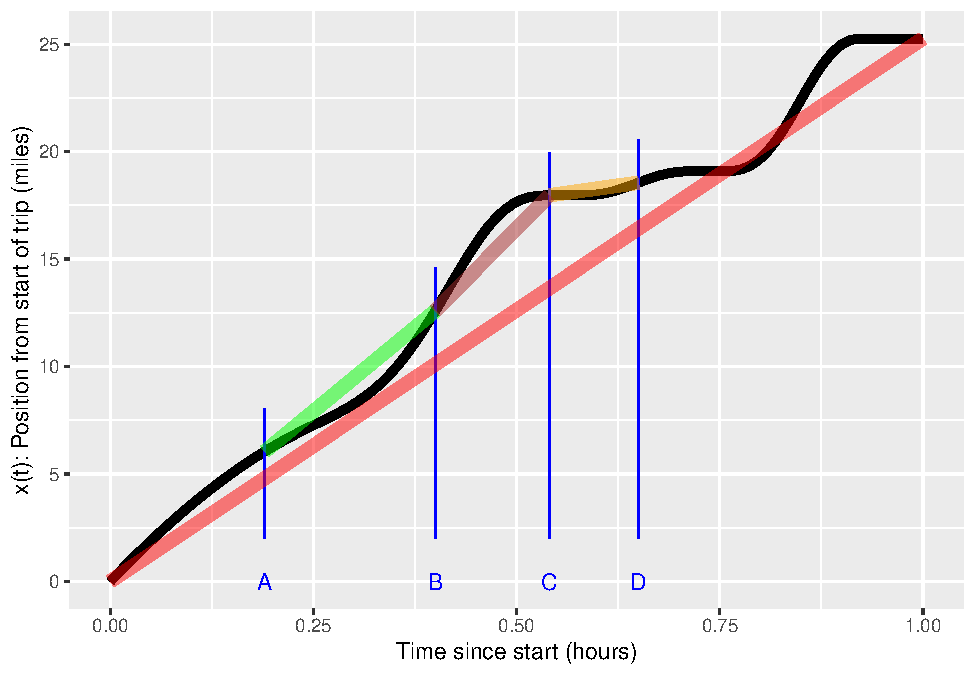
\includegraphics{CalcZ-notes_files/figure-latex/stop-and-go-1.pdf}

During the interval from B to C, the car was travelling relatively fast. The slope of the brown segment connecting the position at times B and C is the \textbf{\emph{average}} rate of change between times B and C. It's easy to see that the average rate of change from B to C is larger than the overall average from \(t=0\) to \(t=1\). Calculating that slope is a matter of evaluating the position at the endpoints and dividing by the length of the interval.

What is the average rate of change in the car's position during the interval \(t_B = 0.40\) to \(t_C=0.54\)?

The length of the interval is \(t_C - t_B = 0.54-0.40=0.14\).

Evaluating the function gives \(x(t_C) = 18\) and \(x(t_B) = 12.6\).

Rise is \(x(t_C) - x(t_B) = 18 - 12.6 = 5.4\).

Run is \(t_C - t_B = 0.54-0.40=0.14\).

The average rate of change during the interval is \$5.4/0.14 = 38.6 \$ miles/hour.

The graph shows a simplified model of the amount of usable wood that can be harvested from a typical tree in a managed forest of Ponderosa Pine. (You can see some actual forestry research models \href{https://www.fs.fed.us/rm/pubs/rmrs_gtr292/1992_milner.pdf}{here}.)

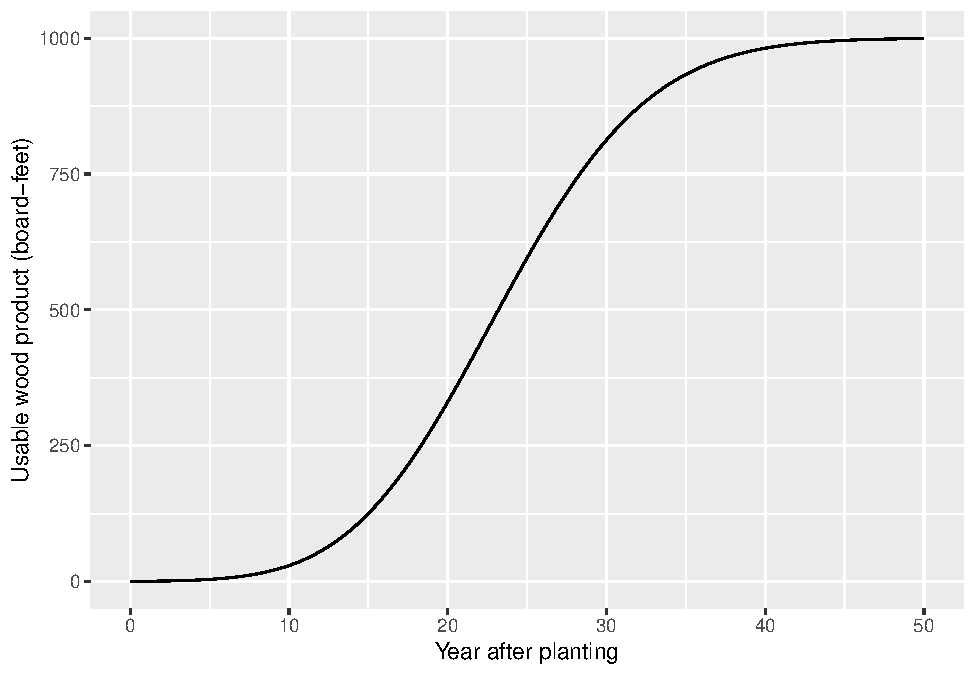
\includegraphics{CalcZ-notes_files/figure-latex/aver-tree-1.pdf}

You are writing a business plan for a proposed pine forest. Among other things, you have to forecast the revenue that will be generated and when you will have salable product.

They say that ``time is money.'' Every year you wait before harvest is another year that you don't have the money. On the other hand, every year that you wait means more wood at the end. How to decide when to harvest?

The tree continues to grow until year 50, when it seems to have reached an equilibrium: perhaps growth goes to zero, or rot balances what growth there is. There's no point waiting until after year 50.

At year 25, the tree is growing as fast as it ever will. You'll get about 600 board-feet of lumber. Should you harvest at year 25? No! That the tree is growing so fast means that you will have a lot more wood at year 26, 27, and so on. The time to harvest is when the growth is getting smaller, so that it's not worth waiting an extra year.

The quantity of interest is the average rate of growth from seedling to harvest. Harvesting at year 25 will give a total change of 600 board feet over 25 years, giving an average rate of change of \(600 \div 25 = 24 \mbox{board-feet-per-year}\). But if you wait until year 35, you'll have about 900 board feet, giving an average rate of change of \$900 \div 35 = 25.7 \mbox{board-feet-per-year}.

We've been presenting the average rate of change as a \textbf{number}: \[\frac{f(t_B) - f(t_A)}{t_B - t_A}\]

But it's helpful to think of it as a \textbf{function} that takes two inputs, which we can call \(t_A\) and \(t_B\):
\[\text{ave_rate_of_change}(t_A, t_B) \equiv \frac{f(t_B) - f(t_A)}{t_B - t_A}\]
This is a very subtle maneuver. The formula is exactly the same, but by writing the quantities \(t_A\) and \(t_B\) as inputs (by putting them in parentheses on the left side), we turn the formula into a function.

Sometimes the average-rate-of-change function presents the information in a clear way.

Back to the forest \ldots{} Here's a graph of the average-rate-of change function. The function has two inputs, but botany dictates that we can only be growing word from the time the seedling is planted. So we'll set \(t_A = 0\) and look at the corresponding \emph{slice} of the function:

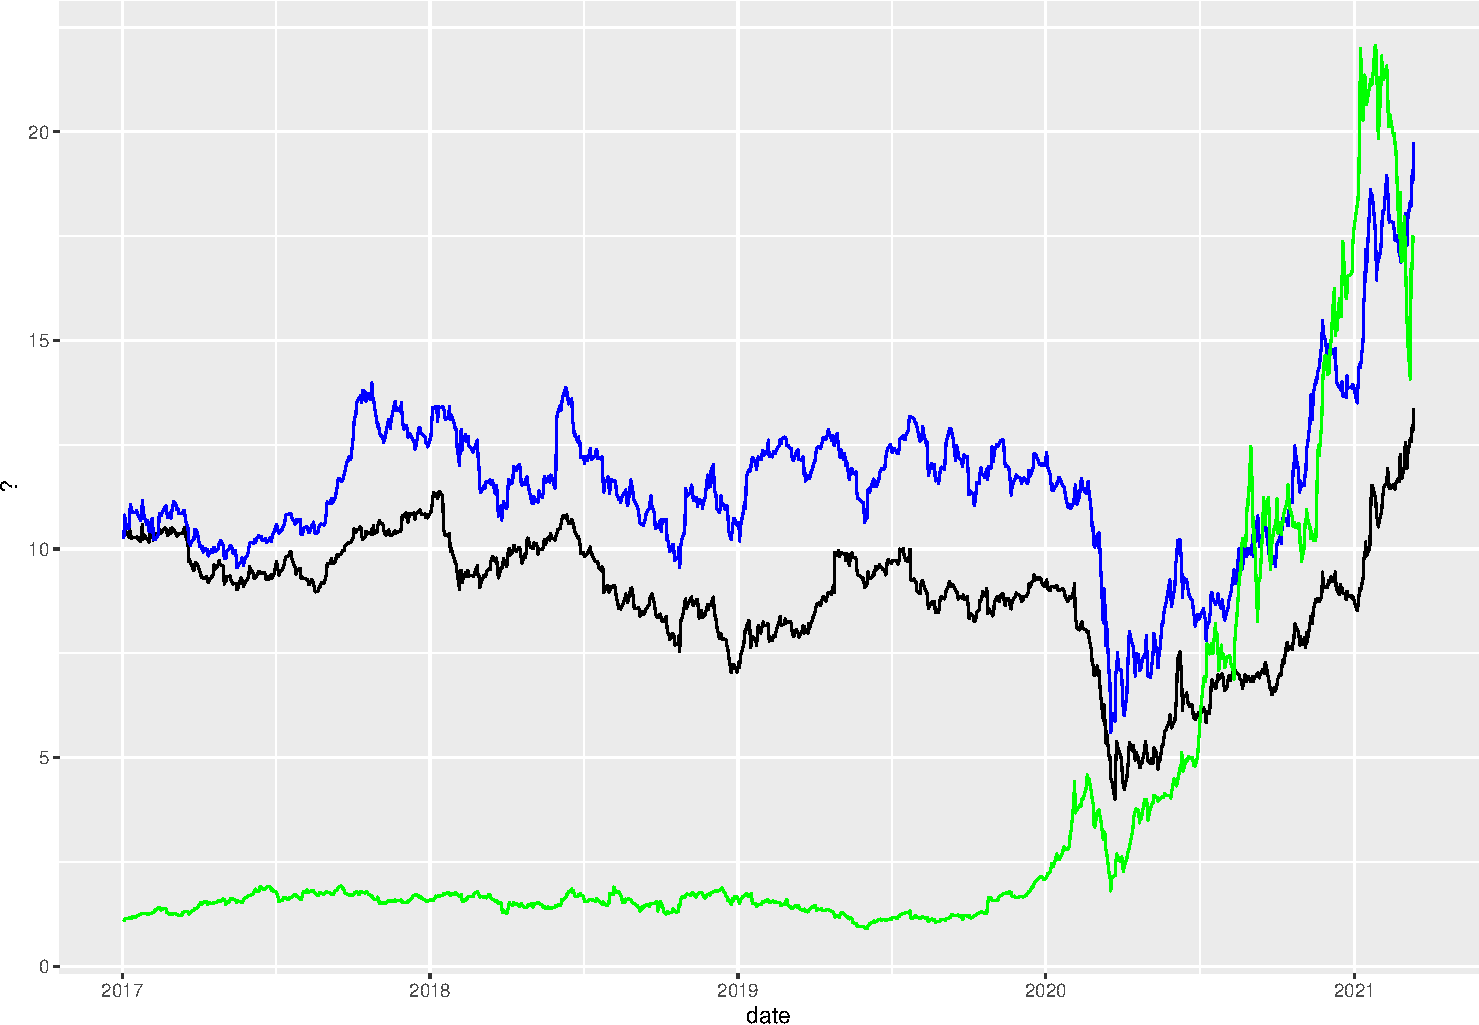
\includegraphics{CalcZ-notes_files/figure-latex/unnamed-chunk-4-1.pdf}
The graph makes it clear that the maximum average growth from planting to harvest will occur at about year 32.

\hypertarget{instantaneous-rate-of-change}{%
\section{Instantaneous rate of change}\label{instantaneous-rate-of-change}}

\begin{enumerate}
\tightlist
\item
  \textbf{{[}Deriv-2b{]}} \emph{Distinguish the ``average rate of change'' from the ``instantaneous rate of change.''}
\end{enumerate}

The car's speedometer shows the speed at each moment---or \textbf{\emph{instant}}---of the trip. As you can see in Figure @ref\{fig:stop-and-go\}, the speed varies and is sometimes less than the average speed, sometimes greater, and occasionally equal to the average speed over the trip. The general term for the kind of quantity presented by the speedometer is the \textbf{\emph{instantaneous rate of change}} of the position function with respect to the input to that function.

Figure @ref\{fig:instant-speed\} shows the instantaneous rate of change of position with respect to time.

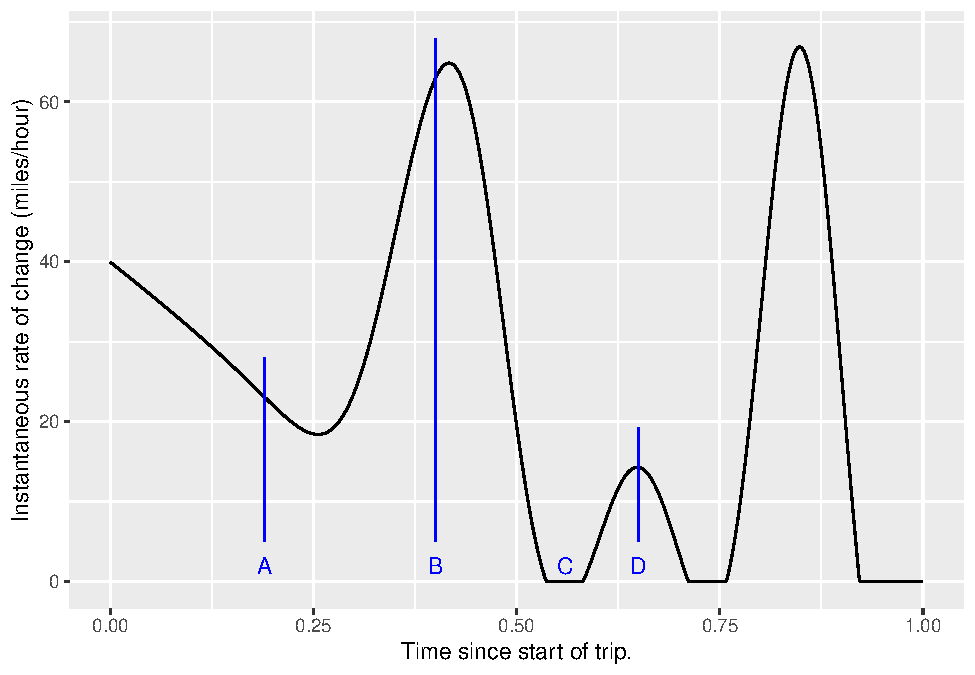
\includegraphics{CalcZ-notes_files/figure-latex/instant-speed-1.pdf}
The two graphs in Figures @ref\{fig:stop-and-go\} and @ref\{fig:instant-speed\} show exactly the same car trip. The presentation of the data in the different graphs makes it easy to see some things and hard to see others. For instance, figuring out when the car is at a stand-still is harder in the position-vs-time graph than in the speed-vs-time graph. This is very much in the spirit of the sand-furrows example at the start of this chapter: it's much easier to perceive the furrows because the lighting highlights areas sloping toward the sun as bright and areas sloping away from the sun as dark. In Figure @ref\{fig:instant-speed\} we're not using light-and-dark for the display. Instead, we're showing the instantaneous speed as the vertical position

Recall that the interval between \(t_B\) and \(t_C\) had an \textbf{\emph{average rate of change}} of about 39 miles-per-hour. Looking at the \textbf{\emph{instantaneous rate of change}} tells the story differently: at time \(t_B\) the car was accelerating to about 60 miles-per-hour. Then it gradually slowed, coming to a stop just before time \(t_C\).

Figure @ref\{fig:stop-and-go\} shows the function \(\mbox{position}(t)\). Figure @ref\{fig:instant-speed\} shows a different function, \(\mbox{speed}(t)\). Although the two functions are different, they are intimately related: \(\mbox{speed}(t)\) is the \textbf{\emph{instantaneous rate of change}} of \(\mbox{position}(t)\).

Two central operations in calculus are:

\begin{enumerate}
\def\labelenumi{\arabic{enumi}.}
\tightlist
\item
  Given a function \(f(t)\), find the function \(g(t)\) giving the instantaneous rate of change of \(f()\). This process of deriving \(g(t)\) from \(f(t)\) is called \textbf{\emph{differentiation}}.
\item
  Given a function \(g(t)\), find the \(f(t)\) of which \(g(t)\) is the instantaneous rate of change. This process of finding \(f()\) given \(g()\) is called \textbf{\emph{anti-differentiation}}.
\end{enumerate}

YOU WERE WORKING HERE.

Sometimes, working with the average-rate-of-growth function directly tells you what you need. Other times, you need to extend your model.

Between year 30 and 32, there is hardly any change in the value of the average-rate-of-change function. It's increasing a little, but is it really worthwhile to wait. One argument is that at year 29 you already have a valuable resource: wood that could be money in the bank. If the money were in the bank, you could invest it and earn more money \emph{and} at the same time get a new seedling in the ground to start its growth. You're doing two things at once. Efficient!

To know what is the best year for harvest from this point of view, you want to calculate the effective ``interest rate'' on the present amount of wood that you earn in the form of new wood. That interest rate is the

\hypertarget{instantaneous-rate-of-change-1}{%
\chapter{Instantaneous rate of change}\label{instantaneous-rate-of-change-1}}

\hypertarget{from-average-to-instant}{%
\section{From average to instant}\label{from-average-to-instant}}

YOU HAVE KNOWN HOW TO CALCULATE AN AVERAGE RATE OF CHANGE for a long time. But possibly you don't yet fully know what the \textbf{use} of such a calculation is other than to help you pass a math test. In this section, we're going to show how to calculate the \textbf{\emph{instantaneous rate of change}} function and show some of the many things this is useful for.

To orient you to what's going to happen \ldots{}

\begin{enumerate}
\def\labelenumi{\arabic{enumi}.}
\tightlist
\item
  We're going to set up the familiar average-rate-of-change calculation in a new framework.
\item
  Using that framework, you'll be able to calculate an average-rate-of-change \emph{function}.
\item
  Then, by turning a knob on the calculation in (2), you'll be able to calculate the \textbf{\emph{instantaneous}} rate of change function. By the way, the knob is called \(h\).
\end{enumerate}

In short, this section will introduce you to the operation called \textbf{\emph{differentiation}}.

\hypertarget{the-h-framework}{%
\section{\texorpdfstring{The \(h\) framework}{The h framework}}\label{the-h-framework}}

Calculating an average rate of change involved specifying an interval of the function domain: the left side \(t_A\) and the right side \(t_B\). Let's change this notation a little:

\begin{itemize}
\tightlist
\item
  Left endpoint of domain: \(t_0\)
\item
  Right endpoint of domain: \(t_0 + h\)
\end{itemize}

There is nothing fundamentally new here. The interval is still specified by two numbers, but now they are called \(t_0\) and \(h\). The width of the interval is just \(h\), which is a little easier to write than \(t_B - t_A\), but is still just the width.

The \textbf{\emph{average rate of change}} in the new notation is \[\frac{f(t_0 + h) - f(t_0)}{h}\ \ \mbox{rather than}\ \ \frac{f(t_B) - f(t_A)}{t_B - t_A}\]

Why are you using \(t\) instead of \(x\)?

Remember, the \emph{name} of an input can be anything at all so long as you use it consistently on the left side of \(\equiv\) and on the right side. All of these are the same definition:
\[g(t) \equiv e^{kt},\ \ g(x) \equiv e^{kx},\ \ g(y) \equiv e^{ky},\ \ g(\mbox{altitude}) \equiv e^{k\,{\small{\text{altitude}}}}\]
When we work with functions of two or more variables, it will be essential to give easily distinguished names to the inputs. We're trying to get you in the habit of paying attention to the names of inputs and break a \emph{bad habit} from high-school math of calling the input \(x\) and the output \(y\).

Now we are going to make a small, subtle, and important change. Instead of thinking of the average rate of change \emph{at a specific interval} \(t_0\) to \(t_0 + h\), we're going to write an average-rate-of-change \textbf{\emph{function}}. And since we're in the habit of giving \emph{names} to functions, we'll be careful to name average-rate-of-change functions in a way that makes explicit the connection to the function \(f(t)\) whose rate of change is being calculated.

Our convention will be to use two additional components in the names of average-rate-of-change functions. The first component is to lead with a ``D'' in a caligraphic font: \(\cal D\). The second component will be the name of the input whose interval is being used in calculating the rate of change. So \ldots{}

\[{\cal D}_t\, f(t) \equiv \frac{f(t + h) - f(t)}{h}\]
You can pronounce \({\cal D}_t\) as ``difference with respect to \(t\).'' But remember that the function name is the whole deal, \({\cal D}_t\, f()\), which is to be read as ``difference with respect to \(t\) of \(f()\).'' Admittedly a long name. Don't be surprised later when we start using \emph{nicknames} like Liz (for Elizabeth) or Bill (for William). For instance, later we'll save ink and breath by using the nickname \(\dot{f}()\) instead of \({\cal D}_t\, f()\).

FOLLOWING NEEDS TO BE SORTED OUT \ldots{}

From the way we've defined \({\cal D}_t f(t)\), it's reasonable to assume that \(h\) is a \textbf{\emph{parameter}}: a symbol naming a numerical value that has to be specified before \({\cal D}_t\, f(t)\) can be evaluated at a specific \(t\).

Find an average-rate-of-change function with respect to \(x\) of \(g(x) \equiv x^2\).

\[{\cal D}_x g(x) = \frac{(x + h)^2 - x^2}{h}\\
= \frac{x^2 + 2 x h + h^2 - x^2}{h}\\
= \frac{2 x h + h^2}{h} = 2 x + h\]

I like to think of \(h\) as a kind of \emph{tire iron}, a small tool used to stretch the bead of a bicycle tire in order to pull it over the wheel rim.

\begin{figure}

{\centering 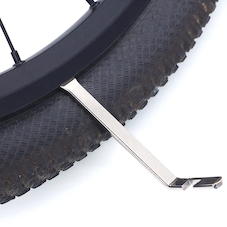
\includegraphics[width=0.3\linewidth]{www/tire-iron}

}

\caption{A tire iron in use}\label{fig:unnamed-chunk-7}
\end{figure}

Once the tire iron has done its job, it's removed and you would never know that it was ever there (except that the tire is now successfully mounted on the wheel).

Find an average-rate-of-change function with respect to \(x\) of \(g(x) \equiv x^2\), but remove the tire iron \(h\) when you're done.

\[{\cal D}_x g(x)
= \frac{(x + h)^2 - x^2}{h}\ \ \mbox{stretch $x$ a bit}\\
= \frac{x^2 + 2 x h + h^2 - x^2}{h}\ \ \mbox{pull over rim}\\
= \frac{2 x h + h^2}{h} \ \ \mbox{still pulling ...}\\
= 2 x + h \ \ \mbox{success!}\]

Now remove the tire iron to get \[{\cal D}_x g(x) = 2x\].

But this is calculus, not bicycle mechanics. How do we know that removing the tire iron isn't damaging the mathematical wheel? Historically, this has been a serious debate, resolved only with great difficulty more than a century after calculus started being used successfully.

Still in the spirit of having fun, let's try a more serious metaphor\ldots{} imagining \(h\) is actually a central character in a calculus play. The character \(h\) is in the middle of the story but \emph{never appears in the play}, like the missing character Godot in the famous play \emph{\href{https://en.wikipedia.org/wiki/Waiting_for_Godot\#Godot}{Waiting for Godot}}.

We said that \(h\) in the finite rate of change function \({\cal D}_x g()\), so long as \(h\) is small, plays both a central role and has hardly any effect. An economizing director re-writes the play to take \(h\) out of it, setting \(h=0\): a non-speaking, offstage role.

We've already seen using legitimate algebra that \[{\cal D}_x g(x) = 2 x + h\] Re-writing by replacing \(h\) with 0 streamlines the play, turning \(\Delta g()\) from a dialog involving both \(x\) and \(h\) into a monologue with \(h\) absent: \[{\cal D}_x g(x) = 2 x\]. Simple.

And yet \ldots{} the director gets a letter from the Bit Players Union.

\begin{quote}
\emph{We observe that you have eliminated the role of \(h\) in the final production version of \({\cal D}_x g(x)\). This is a violation of Union regulations. Recall that the rate-of-change function \({\cal D}_x g(x)\) is defined as a ratio: \[{\cal D}_x g(x) \equiv \frac{g(x+h) - g(x)}{h}\] Although the name \(h\) does not need to appear in the argument list of \({\cal D}_x g(x)\), eliminating \(h\) entirely by replacing her with zero is a \textbf{division by zero error} forbidden by Article 3.16§B¶2 of the Unified Laws of Arithmetic. We ask that you comply with this Article by re-instating the role of \(h\) in all evaluations of \({\cal D} g(x)\).}
\end{quote}

Reading this, the director calls her lawyer. Is there a loophole for removing \(h\) without breaking the mathematical prohibition on dividing by zero?

\hypertarget{the-derivative-operator}{%
\section{The derivative operator}\label{the-derivative-operator}}

Let's put aside for the moment the issue of the disappearing \(h\). Historically, such ``putting aside'' has incurred a great deal of criticism. In 1734, famous philosopher \href{https://en.wikipedia.org/wiki/George_Berkeley}{George Berkeley} (1685-1753) published a long-titled book: \emph{The Analyst: A Discourse Addressed to an Infidel Mathematician: Wherein It Is Examined Whether the Object, Principles, and Inferences of the Modern Analysis Are More Distinctly Conceived, or More Evidently Deduced, Than Religious Mysteries and Points of Faith}. In \emph{The Analyst}, Berkeley took issue with the arguments of that time that it is legitimate to divide by \(h\) when, ultimately, \(h\) will be replaced by zero. Calling \(h\) an ``evanescent increment,'' he asked,

\begin{quote}
\emph{``And what are these same evanescent Increments? They are neither finite Quantities nor Quantities infinitely small, nor yet nothing. May we not call them the ghosts of departed quantities?''}
\end{quote}

Interesting, Berkeley believed that the ghost of \(h\) yielded correct results. His objection was that the framers of calculus had made two, canceling errors.

\begin{quote}
\emph{``{[}B{]}y virtue of a two fold mistake you arrive, though not at science, yet truth.''}
\end{quote}

Berkeley was saying that calculus had not yet been put on a solid logical foundation. It was more than a century after Berkeley's death that this work was accomplished. Once accomplished, the results that had been claimed true all along were confirmed.

I propose that we start with the results, which is what everyone \emph{uses}. Later, we can introduce the new concepts on which the new logic was based. The names of the concepts---continuity, smoothness, singularity---are widely and effectively used in talking about functions, but the names, like many words in English, can be put to good and accurate use without memorizing the precise definitions.

On to the results \ldots{}

\begin{enumerate}
\def\labelenumi{\arabic{enumi}.}
\tightlist
\item
  Every ``smooth'' function \(h(x)\) has a corresponding function that is its derivative \(\partial_x h(x)\).
\item
  Finding the algorithm for \(\partial_x h(x)\), called \textbf{\emph{differentiating \(h()\)}}, is \emph{automatic} in the sense that it can be done by computer without human intervention or judgment.
\item
  When there is an algebraic formula for \(h(x)\), the computer can find the algebraic formula for \(\partial_x h(x)\). This is called \textbf{\emph{symbolic differentiation}}.
\item
  When there is no algebraic formula for \(h()\), the computer can use \textbf{\emph{numerical differentiation}} which involves a non-zero \(h\). The results of numerical differentiation on functions with formulas can differ subtly from the results from symbolic differentiation. Usually the difference is too small to notice, but in extreme cases it is not. It's important for the user of numerical differentiation to know how to identify extreme cases and deal with them.
\end{enumerate}

YOU WERE HERE.

Often, we use a function so briefly that it's not worth naming. For instance, rather than saying

\begin{quote}
``Consider the function \(h(x) = \sin(2\pi x/P)\) and the corresponding average rate of change function \({\cal D}_x h(x)\) \ldots{}''
\end{quote}

We'll write: \({\cal D}_x [\sin(2\pi x/P)]\)

\hypertarget{evanescent-h}{%
\section{\texorpdfstring{Evanescent \(h\)}{Evanescent h}}\label{evanescent-h}}

The word ``evanescent'' means, ``lasting for only a short time, then disappearing quickly and being forgotten.'' (\href{https://dictionary.cambridge.org/us/dictionary/english/evanescent}{Source}) Another dictionary definition is ``tending to vanish like vapor.'' (\href{https://www.merriam-webster.com/dictionary/evanescent}{Source}) I've used metaphors for \(h\): tire irons, dramatic characters who never appear or speak. Here's another one: the solvent in ink or paint. Ink and paint are liquid yet become solid when brushed on a surface. This can happen because the solid pigments are suspended in liquid. Exposed to the air, the liquid vaporizes and is forgotten. The solid pigment remains on the surface.

We can easily evaluate an \textbf{\emph{average rate of change function}}, for instance \({\cal D}_t g(t)\) by evaluating \(g(t)\) at two different inputs and dividing by the distance between the inputs:
\[{\cal D}_t g(t) = \frac{g(t+h) - g(t)}{h}\]
So if you know \(g()\), you know \({\cal D}_t g(t)\). By making \(h\) very small, the ``average'' starts to look like ``instantaneous.'' Over a small interval of length \(h\), every smooth function looks like a straight line. For a straight line, the average rate of change is exactly the same as the instantaneous rate of change.

We'd like to take \(h\) out of the picture, imagining that it is zero but not dealing with ``divide by zero'' if we can avoid it. To signify this idea of neglecting \(h\), we'll use a new notation. Rather than \({\cal D}_t g(t)\) which has that pesky \(h\) in it, we'll write \(\partial_t g(t)\), using the lower-case \(\partial\). The function \(\partial_t g(t)\) can properly be called the \textbf{\emph{instantaneous rate of change}} of \(g(t)\). But everyone calls it the \textbf{\emph{derivative of \(g(t)\) with respect to \(t\)}} Many people leave out the ``with respect to'' part, which I suppose is fine for a function like \(g(t)\) which has only one input. But functions constructed in modeling generally have multiple inputs, so it's a bad habit to neglect to identify which one the derivative is ``with respect to.'' We'll always sneak the ``with respect to'' by putting the little subscript on \(\partial_t\).

We lose something by letting \(h\) vaporize. There is an easy formula for \({\cal D}_t g(t)\), but without \(h\) we can't write down such a formula for the derivative. Mathematicians like to bridge the gap between \({\cal D}\) and \(\partial\), that is between average and instantaneous rates of change, by writing the formula for the derivative with a little ``caution'' sign out front.
\[\partial_t g(t) = \lim_{h\rightarrow 0} \frac{g(t+h) - g(t)}{h}\]
The caution sign is mysterious to newcomers because it is saying something absurd: ``Remember to forget \(h\).''

There are people who do actual calculations with \(\lim_{h\rightarrow 0}\) but nobody needs to any more unless they invent a brand-new function that can't be written with existing functions. If you do happen to invent such a brand-new function, please remember that you should also invent the derivative of that function. Fortunately for us, the inventors of the past have done the work for us. Here's a list of what they found for the mathematical functions that underlie our basic modeling functions:

\begin{itemize}
\tightlist
\item
  \(\partial_x e^x = e^x\)
\item
  \(\partial_x x^0 = 0\)
\item
  \(\partial_x x^p = p\, x^{p-1}\). unless \(p=0\).
\item
  \(\partial_x \sin(x) = \cos(x)\)
\item
  \(\partial_x \cos(x) = -\sin(x)\)
\item
  \(\partial_x \mbox{sigmoid}(x) = \mbox{hump}(x)\)
\end{itemize}

We're going to leave \(\partial_x \mbox{hump}(x)\) alone for now until we have a more complete understanding of derivatives. But other than that, notice that the derivative of every one of these mathematical functions---exponential, power-law, sinusoid---is also in the set of the basic functions.

How can we know that these formulas are right? Let's start by comparing them to the functions computed from the \({\cal D}_x\) formula when \(h\) is very small.

Consider \(\partial_x e^x\), which is claimed to be \(e^x\). Figure @ref\{fig:exp-h\} plots \(e^x\) (in green) as well as a function ARC\((x, h)\) (\textbf{A}verage \textbf{R}ate of \textbf{C}hange) that takes both \(x\) and \(h\) as inputs: \[\mbox{ARC}(x, h) \equiv {\cal D}_x e^x = \frac{e^{x+h} - e^x}{h} = e^x \frac{e^h - 1}{h}\]

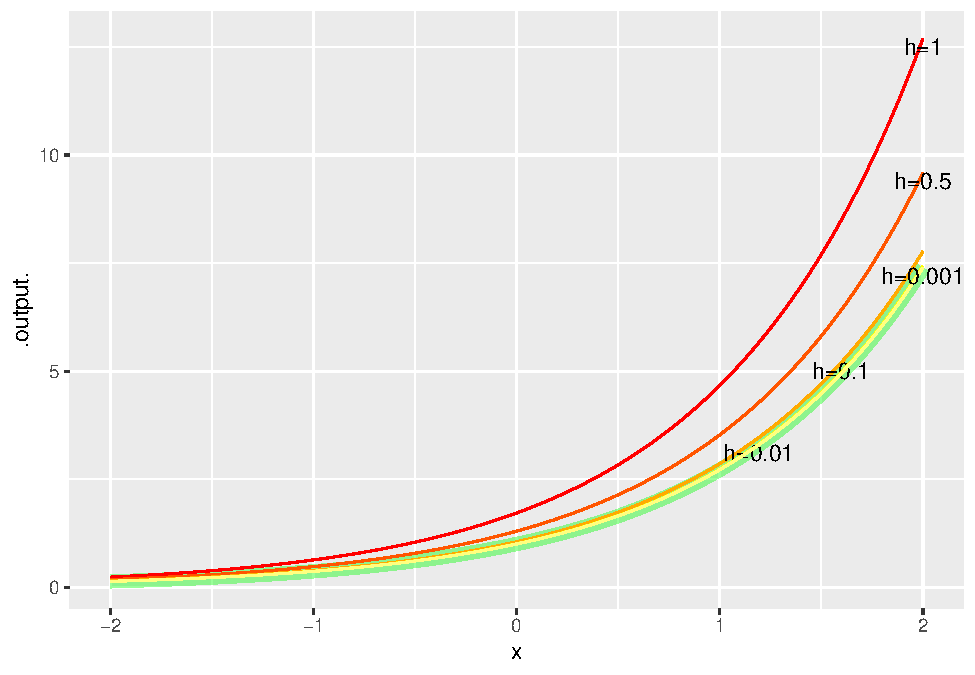
\includegraphics{CalcZ-notes_files/figure-latex/exp-h-1.pdf}

You can see at a glance that \(\mbox{ARC}(x, h)\) gets closer and closer to the claimed derivative, \(e^x\), as \(h\) gets smaller.

A better view of things comes from recognizing that \[\mbox{ARC}(x, h) = e^x \left[\frac{e^h - 1}{h}\right]\]
Let's look at the quantity in brackets as \(h\) gets small. If that goes to 1 for small \(h\), then \(\mbox{ARC}(x, h)\) goes to \(e^x\).

\begin{longtable}[]{@{}ll@{}}
\toprule
\(h\) & \(\frac{e^h - 1}{h}\)\tabularnewline
\midrule
\endhead
1 & 1.71828182845905\tabularnewline
0.1 & 1.05170918075648\tabularnewline
0.01 & 1.00501670841679\tabularnewline
0.001 & 1.00050016670838\tabularnewline
0.0001 & 1.00005000166714\tabularnewline
0.00001 & 1.00000500000696\tabularnewline
0.000001 & 1.00000049996218\tabularnewline
0.0000001 & 1.00000004943368\tabularnewline
0.00000001 & 0.999999993922529\tabularnewline
0.000000001 & 1.00000008274037\tabularnewline
\bottomrule
\end{longtable}

NEXT STEP. The linear expansion \ldots{}

\(f(x + h) \approx f(x) + h \partial_x f(x)\)

D f(g(x)) = f(g(x+h)) - f(g(x)) = f

How we
When we are interested in an \textbf{\emph{instantaneous rate of change function}},

YOU GOT HERE.

\hypertarget{the-delta-operator}{%
\section{\texorpdfstring{The \(\Delta\) operator}{The \textbackslash Delta operator}}\label{the-delta-operator}}

CHANGE THIS TO \({\cal D}\) and introduce it once you have gotten rid of \(h\).

Up until now, we used only functions that take numerical quantities as inputs and produce a numerical quantity as an output. It's time now to broaden our perspective a bit.

Imagine a function named \(\Delta()\) defined like this:
\[\Delta(f) \equiv \frac{f(x+h) - f(x)}{h}\]
\(\Delta()\) takes as input a \textbf{function}. You might have guessed this because the definition uses the name \(f\) for the input to \(\Delta()\), but the name of an input does not matter so long as it is used consistently in the body of the function. Looking at the body, you can that the name \(f\) is being used (twice!) in the position of a function's name.

For instance:

\begin{itemize}
\tightlist
\item
  \(\Delta(\sin) = \frac{\sin(x+h) - \sin(x)}{h}\)
\item
  \(\Delta(x^2) = \frac{(x+h)^2 - x^2}{h}\)
\item
  \(\Delta(a + b x) = \frac{a + b(x + h) - \left(a + b x\right)}{h}\)
\end{itemize}

Why did you use \(=\) in the above statements rather than the \(\equiv\)~?

\(\equiv\) means ``is defined as'' or ``is the name of.'' When we wrote \[\Delta(f) \equiv \frac{f(x+h) - f(x)}{h}\] we were giving a name to a function. But writing \(\Delta(a + b x)\) means to apply the already defined function \(\Delta\) to an input, that input being the straight-line function \(a + b x\). Rather than \emph{defining} what is \(\Delta(a + b x)\) we are \emph{deducing} it from objects that have already been defined.

What is the output of \(\Delta()\)? It takes a \emph{function} as an input and returns \ldots{} a function as an output.

We might choose to give a name to the output, for example fred() or betty() or, more helpfully, \(\mbox{rate}_{\sin}\) or \(\Delta \sin\), but our naming conventions, particularly the use of \(x\) indicate that \frac{\sin(x+h) - \sin(x)}{h}\$ is a function.

In calculus, there are a handful of celebrity functions that take a function as input and return a function as output. Notice that the word ``function'' appeared three times in the previous sentence. To avoid this sort of sleep-inducing repetition, we'll call such functions \textbf{\emph{operators}}.

\begin{quote}
An \textbf{\emph{operator}} (as we will use the word) is a function that, like all functions, has an input and an output. The input is itself a function, the output is also a function, typically (but not always) different from the input.
\end{quote}

\begin{enumerate}
\tightlist
\item
  \textbf{{[}Diff-1a{]}} \emph{Understand the relations between position, velocity, and acceleration as ``change relations.''}
\end{enumerate}

\hypertarget{difference-and-change}{%
\chapter{Difference and change}\label{difference-and-change}}

\begin{verbatim}
Readings: 347-360

Objectives:


#. (Deriv-1b) Know how to calculate the value at a single point of a derivative function.
#. (Deriv-1c) Understand that differentiation is an operator that produces a function called the derivative.
\end{verbatim}

ROUGH ROUGH ROUGH

Lidar measured distance to ground. The function value doesn't really matter. What matters is how the value at a point relates to the values at nearby points. Seeing this difference is how you can spot the Maya ruins.

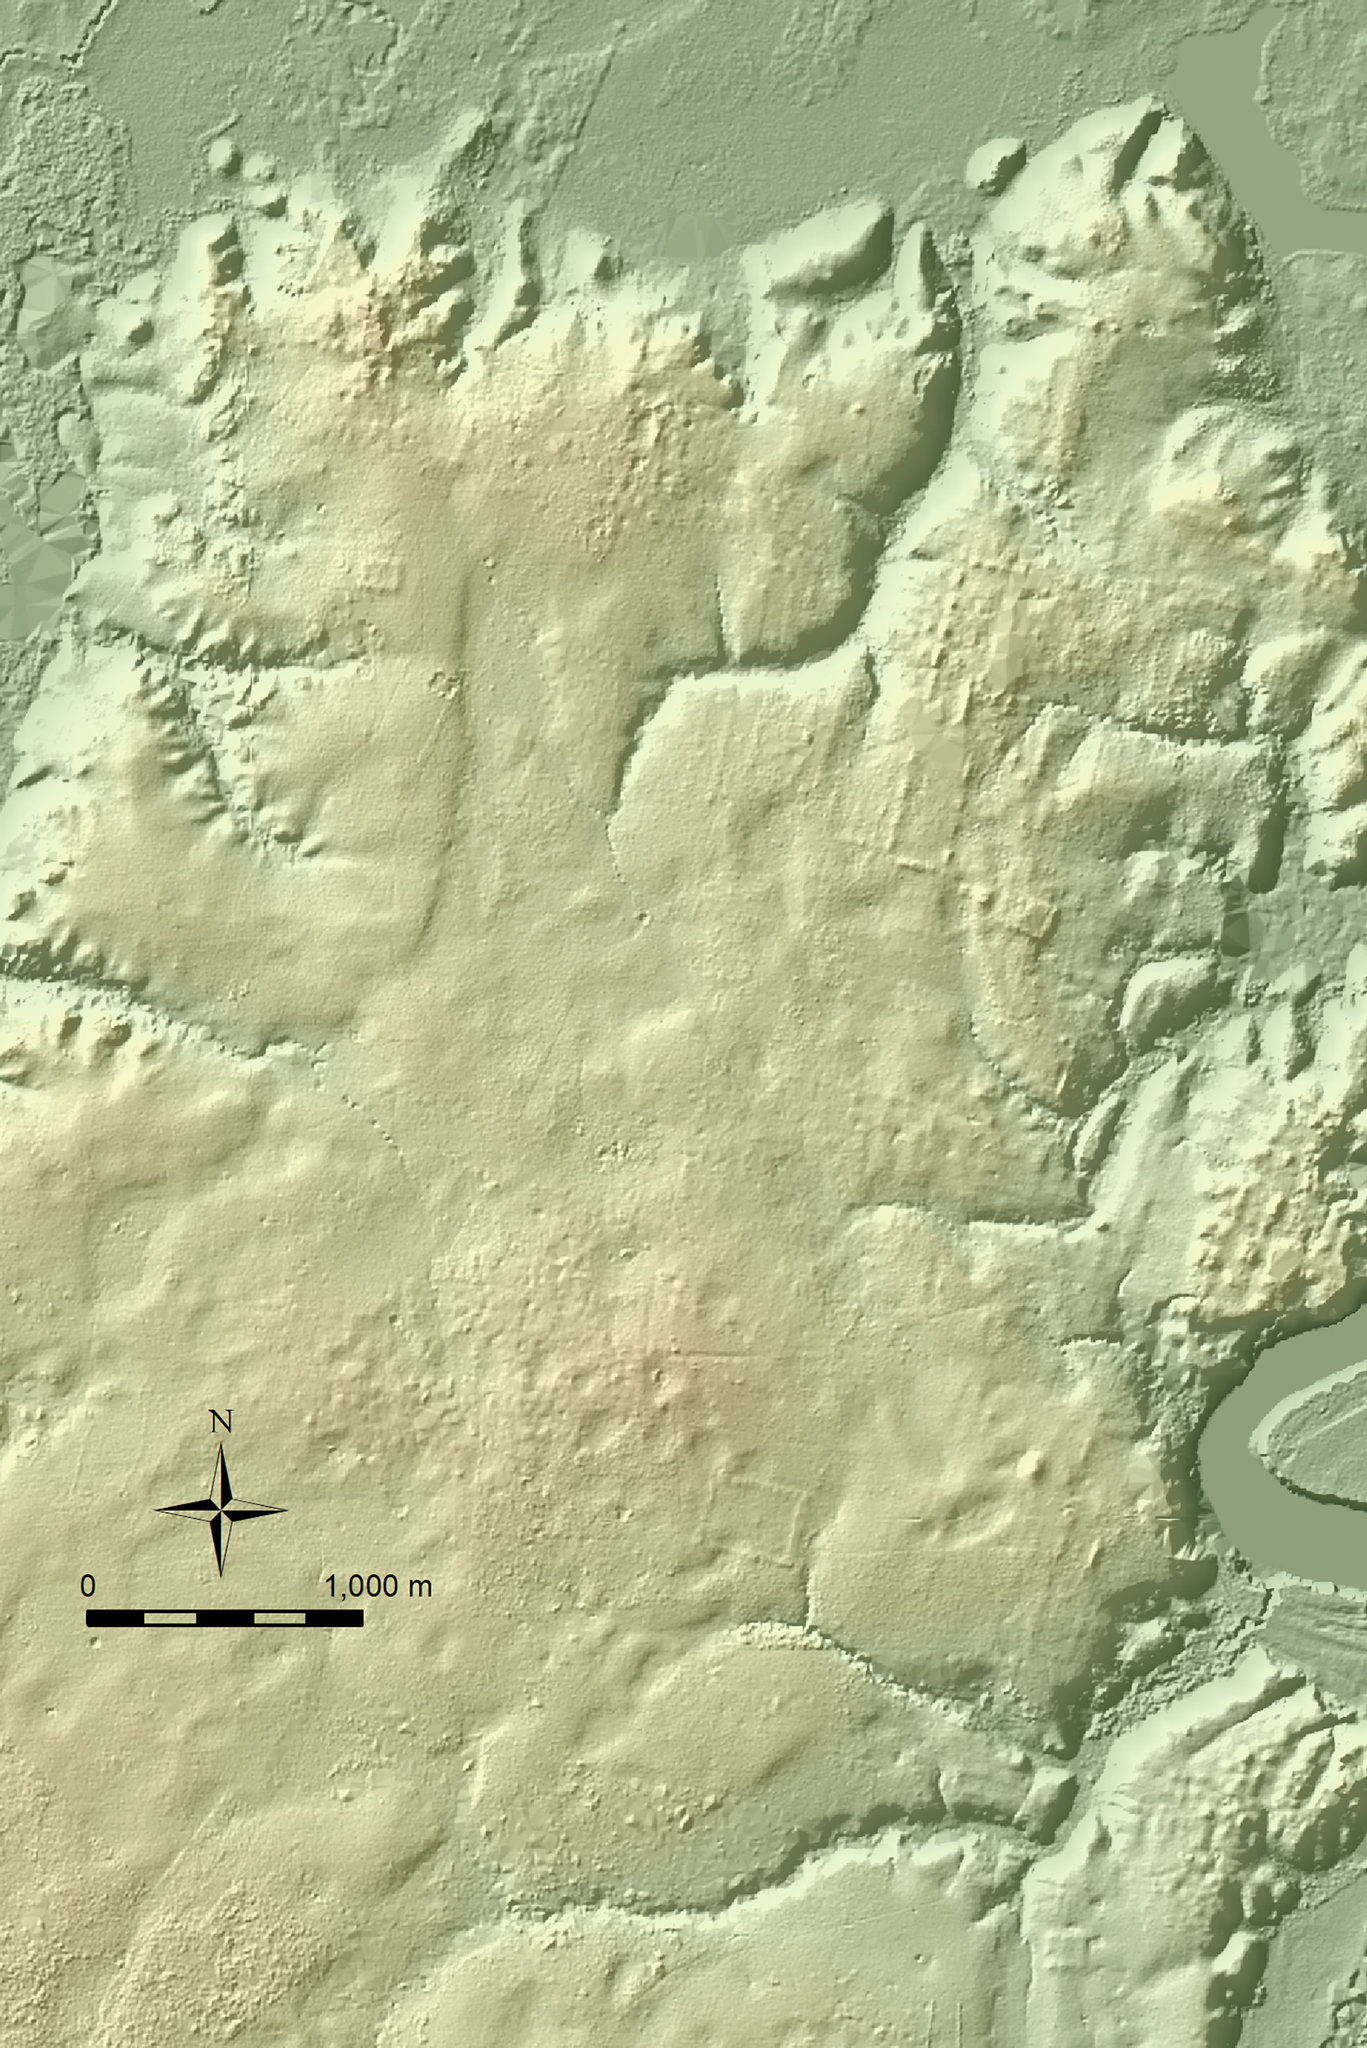
\includegraphics[width=18.99in]{www/mayan-ruins}

Instituto Nacional de Estadística y Geografía/Nacional Center for Airborne Laser Mapping

"The map, published in 2011 by Mexico's National Institute of Statistics and Geography, covered 4,440 square miles in the Mexican states of Tabasco and Chiapas. It was made as part of the institute's mission to create accurate maps to be used by businesses and researchers.

``Dr.~Inomata learned about the map from Rodrigo Liendo, an archaeologist at the National Autonomous University of Mexico. The resolution of the map was low. But the outlines of countless archaeological sites stood out to Dr.~Inomata. So far, he has used it to identify the ruins of 27 previously unknown Maya ceremonial centers that contain a type of construction that archaeologists had never seen before. These sites may hold insights into the origins of Maya civilization.''

\href{https://www.nytimes.com/2019/10/08/science/archaeology-lidar-maya.html}{NYTimes article}

\end{document}
